\documentclass{article}

\usepackage{amsmath,amssymb,amsfonts,amscd,array,amsthm}
\usepackage{subcaption}
\usepackage{mathdots}

\usepackage{pgf,tikz}
    \usetikzlibrary{3d,patterns}
	\usetikzlibrary{arrows}
	\usetikzlibrary{shapes}
	\usetikzlibrary{patterns}
	\usetikzlibrary{calc}
 
\definecolor{orange}{RGB}{255,102,0}
\definecolor{ggreen}{RGB}{0,153,0}
\definecolor{darkblue}{RGB}{0,0,255}
\definecolor{purple}{RGB}{153,51,255}
\definecolor{turq}{RGB}{72,209,204}
\definecolor{gray}{RGB}{220,220,220}

\newcommand\xxaxis{0}
\newcommand\yyaxis{90}
%\newcommand\sq[2]{
%    \fill[fill=gray!30, draw=black, rounded corners, line width=1pt, shift={(\xxaxis:#1)}, shift={(\yyaxis:#2)}] 
%    (0,0) -- (1,0) -- (1,-1) -- (0,-1) -- cycle; }
%
%\newcommand\sqor[2]{
%    \fill[draw=orange, fill=orange!10, line width=1.1pt, rounded corners, shift={(\xxaxis:#1)}, shift={(\yyaxis:#2)}]
%    (0,0) -- (1,0) -- (1,-1) -- (0,-1) -- cycle; }
%\newcommand\sqorhash[2]{
%    \fill[pattern=north east lines, pattern color=orange!35, draw=orange, line width=1.1pt, rounded corners, shift={(\xxaxis:#1)}, shift={(\yyaxis:#2)}]
%    (0,0) -- (1,0) -- (1,-1) -- (0,-1) -- cycle; }
%\newcommand\sqorcheck[2]{
%    \fill[pattern=checkerboard, pattern color=orange!06, draw=orange, line width=1.1pt, rounded corners, shift={(\xxaxis:#1)}, shift={(\yyaxis:#2)}]
%    (0,0) -- (1,0) -- (1,-1) -- (0,-1) -- cycle; }
%
%\newcommand\sqgr[2]{
%    \fill[draw=ggreen, fill=ggreen!05, line width=1.1pt, rounded corners, shift={(\xxaxis:#1)}, shift={(\yyaxis:#2)}]
%    (0,0) -- (1,0) -- (1,-1) -- (0,-1) -- cycle; }
%\newcommand\sqgrhash[2]{
%    \fill[pattern=north east lines, pattern color=ggreen!35, draw=ggreen, line width=1.1pt, rounded corners, shift={(\xxaxis:#1)}, shift={(\yyaxis:#2)}]
%    (0,0) -- (1,0) -- (1,-1) -- (0,-1) -- cycle; }
%\newcommand\sqgrcheck[2]{
%    \fill[pattern=checkerboard, pattern color=ggreen!06, draw=ggreen, line width=1.1pt, rounded corners, shift={(\xxaxis:#1)}, shift={(\yyaxis:#2)}]
%    (0,0) -- (1,0) -- (1,-1) -- (0,-1) -- cycle; }
%
%\newcommand\sqp[2]{
%    \fill[draw=purple, fill=purple!08, line width=1.1pt, rounded corners, shift={(\xxaxis:#1)}, shift={(\yyaxis:#2)}]
%    (0,0) -- (1,0) -- (1,-1) -- (0,-1) -- cycle; }
%\newcommand\sqphash[2]{
%    \fill[pattern=north east lines, pattern color=purple!35, draw=purple, line width=1.1pt, rounded corners, shift={(\xxaxis:#1)}, shift={(\yyaxis:#2)}]
%    (0,0) -- (1,0) -- (1,-1) -- (0,-1) -- cycle; }
%\newcommand\sqpcheck[2]{
%    \fill[pattern=checkerboard, pattern color=purple!06, draw=purple, line width=1.1pt, rounded corners, shift={(\xxaxis:#1)}, shift={(\yyaxis:#2)}]
%    (0,0) -- (1,0) -- (1,-1) -- (0,-1) -- cycle; }
%
%\newcommand\sqbl[2]{
%    \fill[draw=darkblue, fill=darkblue!05, line width=1.1pt, rounded corners, shift={(\xxaxis:#1)}, shift={(\yyaxis:#2)}]
%    (0,0) -- (1,0) -- (1,-1) -- (0,-1) -- cycle; }
%\newcommand\sqblhash[2]{
%    \fill[pattern=north east lines, pattern color=darkblue!35, draw=darkblue, line width=1.1pt, rounded corners, shift={(\xxaxis:#1)}, shift={(\yyaxis:#2)}]
%    (0,0) -- (1,0) -- (1,-1) -- (0,-1) -- cycle; }
%\newcommand\sqblcheck[2]{
%    \fill[pattern=checkerboard, pattern color=darkblue!06, draw=darkblue, line width=1.1pt, rounded corners, shift={(\xxaxis:#1)}, shift={(\yyaxis:#2)}]
%    (0,0) -- (1,0) -- (1,-1) -- (0,-1) -- cycle; }
%    
%\newcommand\sqm[2]{
%    \fill[draw=magenta, fill=magenta!08, line width=1.1pt, rounded corners, shift={(\xxaxis:#1)}, shift={(\yyaxis:#2)}]
%    (0,0) -- (1,0) -- (1,-1) -- (0,-1) -- cycle; }
%\newcommand\sqmhash[2]{
%    \fill[pattern=north east lines, pattern color=magenta!35, draw=magenta, line width=1.1pt, rounded corners, shift={(\xxaxis:#1)}, shift={(\yyaxis:#2)}]
%    (0,0) -- (1,0) -- (1,-1) -- (0,-1) -- cycle; }
%
%% The empty square
%\newcommand\bsq[2]{
%    \fill[fill=white, dotted, draw=black, line width=0.5pt, rounded corners, shift={(\xxaxis:#1)},shift={(\yyaxis:#2)}]
%    (0.05,-0.05) -- (0.95,-0.05) -- (0.95,-0.95) -- (0.05,-0.95) -- cycle; }

%% Kirsten's code %%

% The square
\newcommand\sq[2]{
  \fill[fill=cyan!30, draw=black, rounded corners, line width=1pt, shift={(\xxaxis:#1)},shift={(\yyaxis:#2)}] (0,0) -- (2,0) -- (2,-2) -- (0,-2) --cycle;
}

\newcommand\nsq[3]{
<<<<<<< HEAD
  \fill[fill=cyan!30, draw=black, rounded corners, line width=1pt, shift={(\xxaxis:#1)},shift={(\yyaxis:#2)}] (0,0) -- (2,0) -- (2,-2) -- (0,-2) --cycle;
=======
  \fill[fill=cyan!30, draw=black, rounded corners, line width=1pt, shift={(\xxaxis:#1)},shift={(\yyaxis:#2)}] (0,0) -- (2,0) -- (2,-2) -- (0,-2) --cycle;
>>>>>>> origin/master
\node at (#1+1,#2-1) {$#3$};
}

% colored square
\newcommand\csq[2]{
  \fill[fill=magenta, draw=black,rounded corners, shift={(\xxaxis:#1)},shift={(\yyaxis:#2)}] (0,0) -- (1,0) -- (1,-1) -- (0,-1) --(0,0);
}

% The empty square
\newcommand\bsq[2]{
  \fill[fill=white, fill opacity=0.5, densely dashed, draw=black, rounded corners, shift={(\xxaxis:#1)},shift={(\yyaxis:#2)}] (0,0) -- (1,0) -- (1,-1) -- (0,-1) --(0,0);
<<<<<<< HEAD
}

\begin{document}



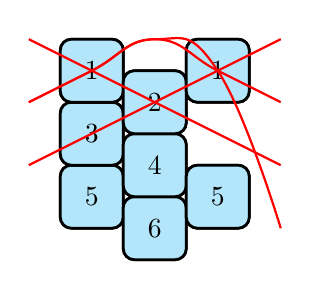
\begin{tikzpicture}[scale=0.4]
\nsq{0}{0}{5};
\nsq{0}{2}{3};
\nsq{0}{4}{1};
\nsq{2}{-1}{6};
\nsq{2}{1}{4};
\nsq{2}{3}{2};
\nsq{4}{0}{5};
\nsq{4}{4}{1};

%\draw [gray!50]  (0,0) -- (1,1) -- (3,1) -- (1,0)  -- (2,-1) -- cycle;
%\draw [red] plot [smooth cycle] coordinates {(0,0) (1,1) (3,1) (1,0) (2,-1)};
%
%\draw [gray!50, xshift=4cm]  (0,0) -- (1,1) -- (2,-2) -- (3,0);
\draw [red,thick] plot [smooth, tension=0.8] coordinates { (7,4) (5,3) (3,2) (1,1) (-1,0)};
\draw [red,thick] plot [smooth, tension=0.8] coordinates { (7,2) (5,3) (3,4) (1,3) (-1,2)};
\draw [red,thick] plot [smooth, tension=0.8] coordinates { (7,0) (3,2) (1,3) (-1,4)};
\draw [red,thick] plot [smooth, tension=0.8] coordinates { (7,-2) (5,3) (3,4) (1,3) (-1,2)};
\end{tikzpicture}


%\begin{center} \begin{tikzpicture}
%    \sqbl{0}{9};    \node at (0.5,8.5)   {\scalebox{0.85}{$1$}};
%    \sqbl{0.5}{8};  \node at (1,7.5)     {\scalebox{0.85}{$2$}};
%                    \node at (1.8,6.6)   {$\ddots$};
%    \sqbl{2}{6};    \node at (2.5,5.5)   {\scalebox{0.85}{$k$}};
%    \sqbl{3}{6};    \node at (3.5,5.5)   {\scalebox{0.85}{$k+2$}};
%    \sqbl{3.5}{5};  \node at (4,4.5)     {\scalebox{0.85}{$k+3$}};
%                    \node at (4.8,3.65)  {$\ddots$};
%    \sqbl{5}{3};    \node at (5.5,2.5)   {\scalebox{0.85}{$k'$}};
%    \sqbl{5.5}{2};  \node at (6,1.5)     {\scalebox{0.85}{$k'+1$}};
%
%    \sqor{2.5}{7};  \node at (3,6.5)     {\scalebox{0.85}{$k+1$}};
%                    \node at (2.25,7.6)  {$\ddots$};
%    \sqor{1}{9};    \node at (1.5,8.5)   {\scalebox{0.85}{$3$}};
%    \sqor{0.5}{10}; \node at (1,9.5)     {\scalebox{0.85}{$2$}};
%    \sqor{0}{11};   \node at (0.5,10.5)  {\scalebox{0.85}{$1$}};
%    \sqor{3}{8};    \node at (3.5,7.5)   {\scalebox{0.85}{$k+2$}};
%                    \node at (2.75,8.6)  {$\ddots$};
%    \sqor{1.5}{10}; \node at (2,9.5)     {\scalebox{0.85}{$4$}};
%    \sqor{1}{11};   \node at (1.5,10.5)  {\scalebox{0.85}{$3$}};
%    \sqor{0.5}{12}; \node at (1,11.5)    {\scalebox{0.85}{$2$}};
%                    \node at (2,12.5)    {$\iddots$};
%                    \node at (4.5,8.5)   {$\iddots$};
%                    \node at (3,11.5)    {$\iddots$};
%                    \node at (5.1,11.6)  {$\ddots$};
%                    \node at (4,10.5)    {$\cdots$};
%                    \node at (4,9.5)     {$\cdots$};
%    \sqor{3}{14};   \node at (3.5,13.5)  {\scalebox{0.85}{$m+1$}};
%    \sqor{3.5}{13}; \node at (4,12.5)    {\scalebox{0.85}{$m+2$}};
%    \sqor{5.5}{11}; \node at (6,10.5)    {\scalebox{0.85}{$k'+1$}};
%    \sqor{5}{10};   \node at (5.5,9.5)   {\scalebox{0.85}{$k'$}};
%    
%    \sqgr{2.5}{5};  \node at (3,4.5)     {\scalebox{0.85}{$k+1$}};
%    \sqgr{2}{4};    \node at (2.5,3.5)   {\scalebox{0.85}{$k$}};
%    \sqgr{3}{4};    \node at (3.5,3.5)   {\scalebox{0.85}{$k+2$}};
%                    
%    \sqgr{4.5}{2};  \node at (5,1.5)     {\scalebox{0.85}{$k'-1$}};
%    \sqgr{5}{1};    \node at (5.5,0.5)   {\scalebox{0.85}{$k'$}};
%                    \node at (4.8,-1)    {$\iddots$};
%    \sqgr{0.5}{2};  \node at (1,1.5)     {\scalebox{0.85}{$2$}};
%    \sqgr{0}{1};    \node at (0.5,0.5)   {\scalebox{0.85}{$1$}};
%    \sqgr{1}{1};    \node at (1.5,0.5)   {\scalebox{0.85}{$3$}};
%    \sqgr{0.5}{0};  \node at (1,-0.5)    {\scalebox{0.85}{$2$}};
%    \sqgr{1.5}{2};  \node at (2,1.5)     {\scalebox{0.85}{$4$}};
%                    \node at (2,-1.5)    {$\ddots$};
%    \sqgr{3}{-2};   \node at (3.5,-2.5)  {\scalebox{0.85}{$m+1$}};
%                    \node at (1.8,2.5)   {$\iddots$};
%                    \node at (2.8,2.5)   {$\iddots$};
%                    \node at (3.5,1.5)   {$\cdots$};
%                    \node at (3.5,0.5)   {$\cdots$};
%                    \node at (3.5,-0.5)  {$\cdots$};
%                    \node at (4.3,2.5)   {$\ddots$};
%\end{tikzpicture} \end{center}
%
%\pagebreak
%
%\begin{figure}[h!] \centering \begin{tikzpicture}%[scale=0.85]
%    \sqor{0}{10};       \node at (0.5,9.5) {\footnotesize $3$};
%    \sqor{0.5}{9};      \node at (1,8.5)   {\footnotesize $4$};
%    \sqor{1}{8};        \node at (1.5,7.5) {\footnotesize $5$};
%    \sqor{1.5}{7};      \node at (2,6.5)   {\footnotesize $6$};
%    \sqorhash{2}{6};    \node at (2.5,5.5) {\footnotesize $7$};
%    \sqbl{0}{8};        \node at (0.5,7.5) {\footnotesize $3$};
%    \sqbl{0.5}{7};      \node at (1,6.5)   {\footnotesize $4$};
%    \sqbl{1}{6};        \node at (1.5,5.5) {\footnotesize $5$};
%    \sqblhash{1.5}{5};  \node at (2,4.5)   {\footnotesize $6$};
%    \sqgrhash{2}{4};    \node at (2.5,3.5) {\footnotesize $7$};
%    \sqgrhash{1.5}{3};  \node at (2,2.5)   {\footnotesize $6$};
%    \sqgr{1}{2};        \node at (1.5,1.5) {\footnotesize $5$};
%    \sqgr{0.5}{1};      \node at (1,0.5)   {\footnotesize $4$};
%    \sqgr{0}{0};        \node at (0.5,-0.5){\footnotesize $3$};
%\end{tikzpicture}
%\caption{}\label{fig:slideexheap1}
%\end{figure}
%
\end{document}
=======
}

\begin{document}

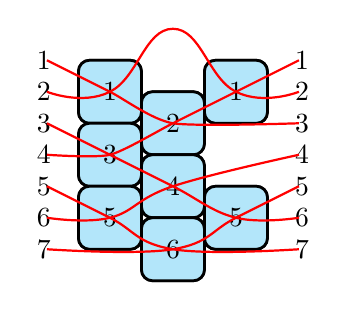
\begin{tikzpicture}[scale=0.4]
\nsq{0}{4}{1};
\nsq{0}{2}{3};
\nsq{0}{0}{5};
\nsq{2}{3}{2};
\nsq{2}{1}{4};
\nsq{2}{-1}{6};
\nsq{4}{4}{1};
\nsq{4}{0}{5};

\node at (7.1,4) {$1$};
\node at (7.1,3) {$2$};
\node at (7.1,2) {$3$};
\node at (7.1,1) {$4$};
\node at (7.1,0) {$5$};
\node at (7.1,-1) {$6$};
\node at (7.1,-2) {$7$};

\node at (-1.1,4) {$1$};
\node at (-1.1,3) {$2$};
\node at (-1.1,2) {$3$};
\node at (-1.1,1) {$4$};
\node at (-1.1,0) {$5$};
\node at (-1.1,-1) {$6$};
\node at (-1.1,-2) {$7$};

%\draw [gray!50, xshift=4cm]  (0,0) -- (1,1) -- (2,-2) -- (3,0);
\draw [red, thick] plot [smooth, tension=.40] coordinates { (7,4) (5,3) (3,2) (1,1) (-1,1)};
\draw [red, thick] plot [smooth, tension=.80] coordinates { (7,3) (5,3) (3,5) (1,3) (-1,3)};
\draw [red, thick] plot [smooth, tension=.40] coordinates { (7,2) (3,2) (1,3)  (-1,4)};
\draw [red, thick] plot [smooth, tension=.70] coordinates { (7,1) (3,0) (1,-1) (-1,-1)};
\draw [red, thick] plot [smooth, tension=.70] coordinates { (7,0) (5,-1) (3,-2) (-1,-2)};
\draw [red, thick] plot [smooth, tension=.70] coordinates { (7,-1) (5,-1) (3,0) (1,1) (-1,2)};
\draw [red, thick] plot [smooth, tension=.70] coordinates { (7,-2) (3,-2) (1,-1) (-1,0)};

\end{tikzpicture}



\end{document}
>>>>>>> origin/master
